%% The following is a directive for TeXShop to indicate the main file
%%!TEX root = diss.tex

\chapter{Motivation}
\label{ch:Motivation}
Deduplication and base delta immediate compression work on two different domains, one is inter-line and works on a cache line granularity while the other works intra-line with a granularity of two, four, or eight bytes. This means that they can both be combined to deduplicate similar lines and compress each of those lines at the same time.

\section{Analysis}
\label{Analysis}
We look at four different benchmarks with different cache patterns and behaviours. One benchmark is very compressible by BDI, the second is compressible using deduplication, the third and fourth are completely incompressible and compressible by both, respectively. We analyze how these benchmarks respond to each type of compression and how a combination of both compression techniques can improve on them.\par
The four benchmarks are:
\begin{figure}
    \begin{subfigure}{\textwidth}
        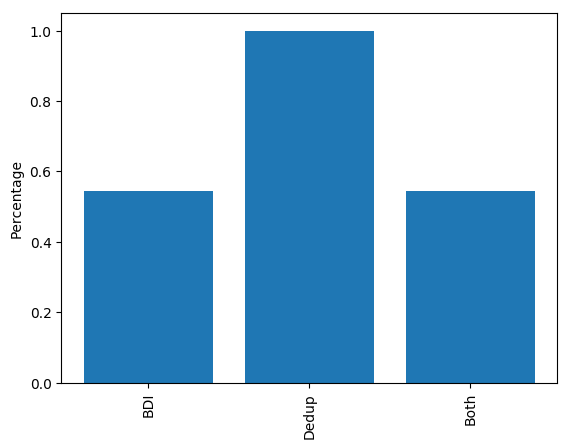
\includegraphics[width=\textwidth]{inversek2j.png}
        \caption{inversek2j}
        \label{fig:inversek2j}
    \end{subfigure}
    \begin{subfigure}{\textwidth}
        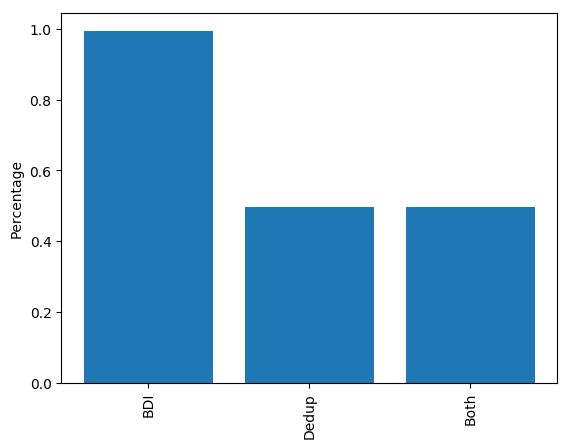
\includegraphics[width=\textwidth]{dedup.png}
        \caption{dedup}
        \label{fig:dedup}
    \end{subfigure}
    \caption[Compression in benchmarks1]{The figure shows the percentage of compressed data compared to original cache sizes.}
\end{figure}
\begin{figure}
    \begin{subfigure}{\textwidth}
        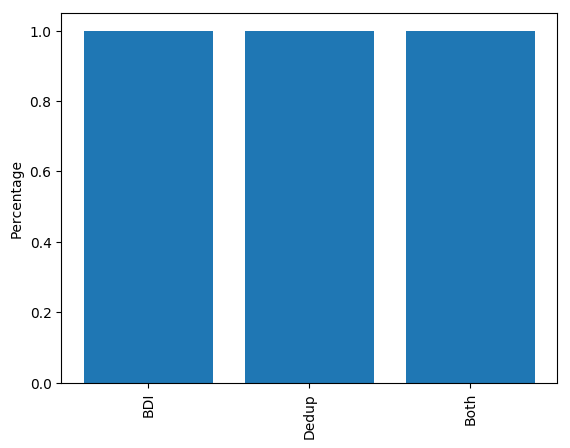
\includegraphics[width=\textwidth]{jmeint.png}
        \caption{jmeint}
        \label{fig:jmeint}
    \end{subfigure}
    \begin{subfigure}{\textwidth}
        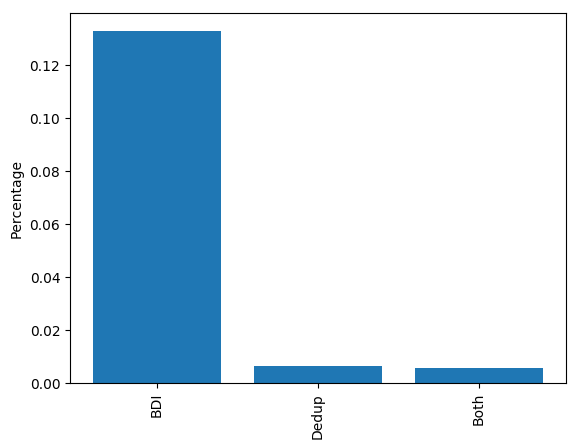
\includegraphics[width=\textwidth]{bwaves.png}
        \caption{bwaves}
        \label{fig:bwaves}
    \end{subfigure}
    \caption[Compression in benchmarks2]{The figure shows the percentage of compressed data compared to original cache sizes.}
\end{figure}
\begin{itemize}
    \item \textbf{inversek2j:} The inversek2j benchmark\cite{axbench} is used in robotic and animation applications. It uses the kinematic equation to compute the angles of 2-joint robotic arms. It deals with arrays of floats that represent angles. Inversek2j is BDI sensitive but doesn't have enough potential to benifit from deudplication. Figure \ref{fig:inversek2j} shows the Dedup, BDI, and Dedup+BDI compressed data size of inversek2j cache dumps as a percentage of the original size.
    \item \textbf{dedup:} The dedup benchmark\cite{parsec} compresses data streams with deduplication. It treats data as integer arrays, divides them into chunks, then tries to build a dictionary out of those chunks and use them for compression. The dedup benchmark is deduplication sensitive. Figure \ref{fig:dedup} shows the Dedup, BDI, and Dedup+BDI compressed data size of dedup cache dumps as a percentage of the original size.
    \item \textbf{jmeint:} The jmeint benchmark\cite{axbench} is a triangle intersection workload that is used in 3d gaming. It takes coordinates of two triangles as its input. This makes most of the data insensitive to BDI compression and deduplication. Figure \ref{fig:jmeint} shows the Dedup, BDI, and Dedup+BDI compressed data size of jmeint cache dumps as a percentage of the original size.
    \item \textbf{bwaves:} The bwaves benchmark\cite{spec} simulates a spherical blast wave. It also contains (at least at the first few cache dumps) a lot of zero lines which are 2D compressible through deduplication and BDI. Figure \ref{fig:bwaves} shows the Dedup, BDI, and Dedup+BDI compressed data size of bwaves cache dumps as a percentage of the original size.
\end{itemize}

\section{Generalization}
\label{Generalization}

\begin{figure}
    \begin{subfigure}[t]{\textwidth}
        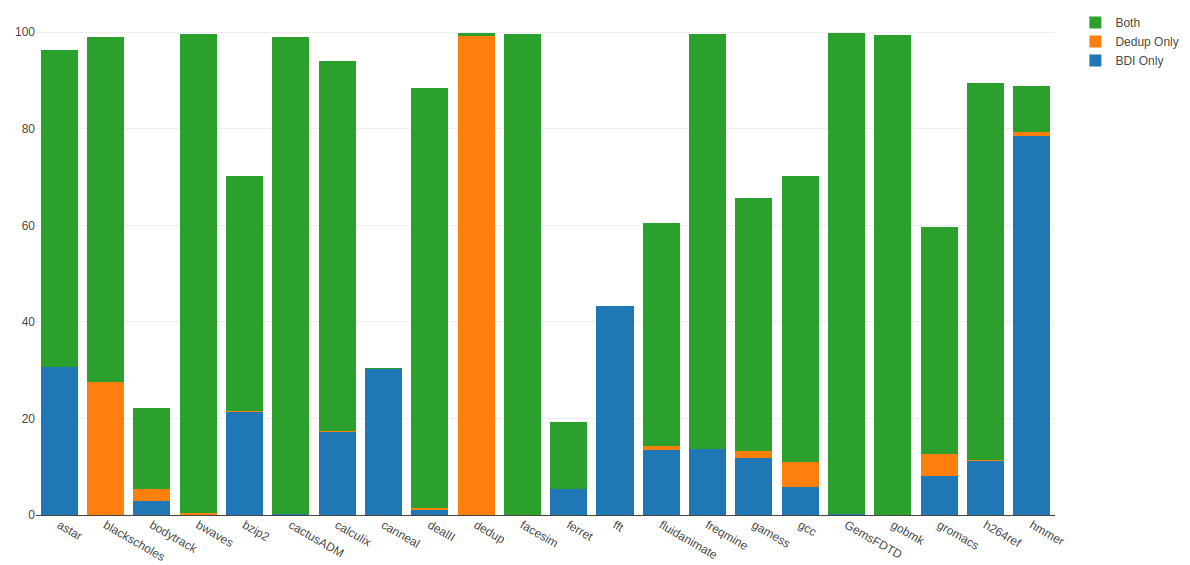
\includegraphics[width=\textwidth]{CompPotential1.png}
    \end{subfigure}
    \begin{subfigure}[b]{\textwidth}
        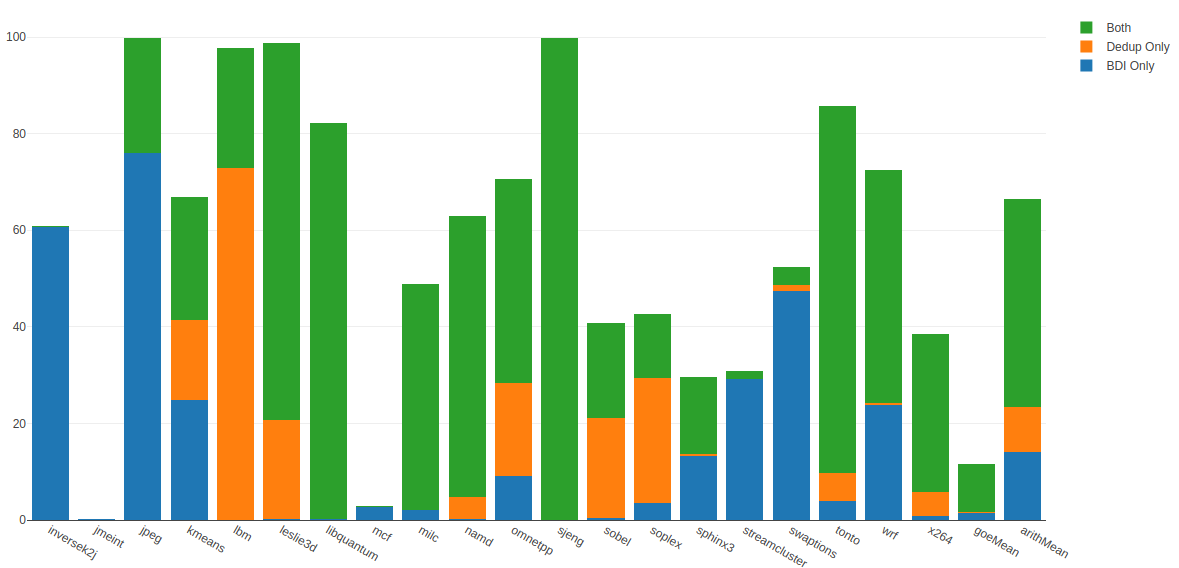
\includegraphics[width=\textwidth]{CompPotential2.png}
    \end{subfigure}
    \caption[Compressible lines]{The figure shows the percentage of cache lines that can be compressed using Dedup, BDI, or both techniques combined together.}
    \label{fig:CompPossibility}
\end{figure}

Generalizing on what we found on the previous section. We used the same cache dumps to create Figure \ref{fig:CompPossibility} showing the percentage of cache lines that can be compressed by BDI, the percentage of cache lines that are similar and thus deduplicable, and the percentage of cache lines that can be compressed using both schemes.\par
As Figure \ref{fig:CompPossibility} shows, BDI and Deduplications are orthogonal to some degree. The existence of some cache lines that can be compressed by only one of both compression schemes means they can work separately without affecting each other. However, because there are lines that can be compressed by both schemes, BDI can lose some of it's improvements because of deduplication. For example, if ten lines were similar and compressible by BDI, using BDI will compress each of them on it's own, using deduplication will reduce all ten lines to only one line. Using both techniques means deduplication still compresses ten lines to one, but BDI now compresses only one line instead of 10. The improvements of BDI can thus be limited by deduplication.\par
\begin{figure}
    \begin{subfigure}[t]{\textwidth}
        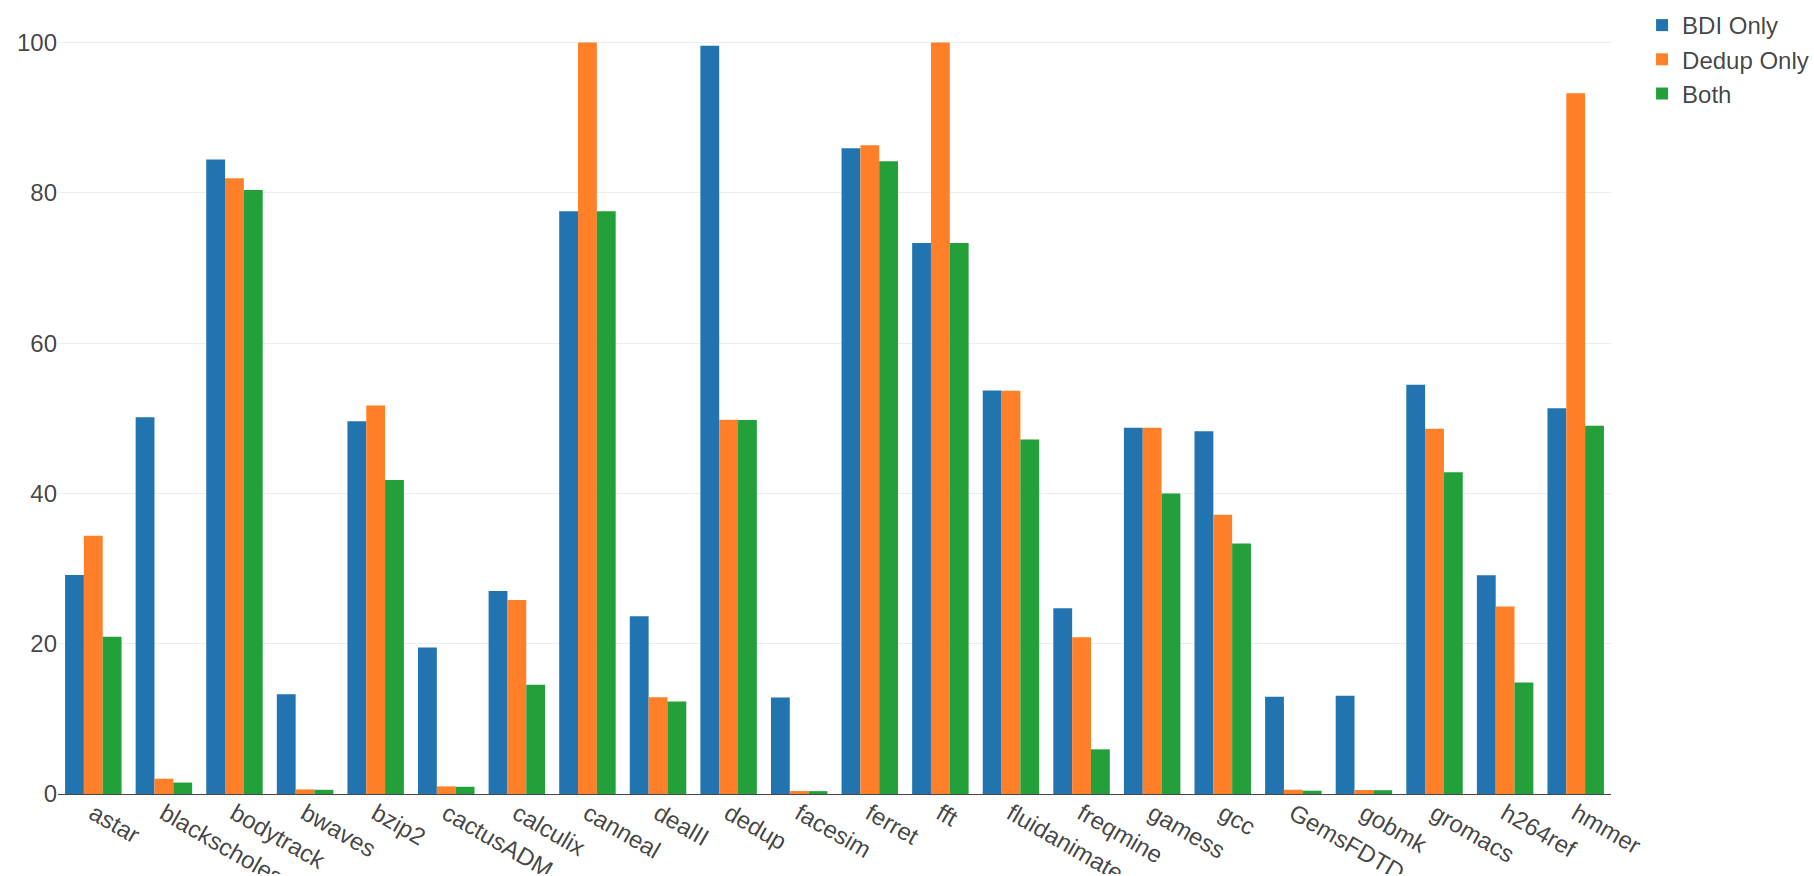
\includegraphics[width=\textwidth]{CompSize1.png}
    \end{subfigure}
    \begin{subfigure}[b]{\textwidth}
        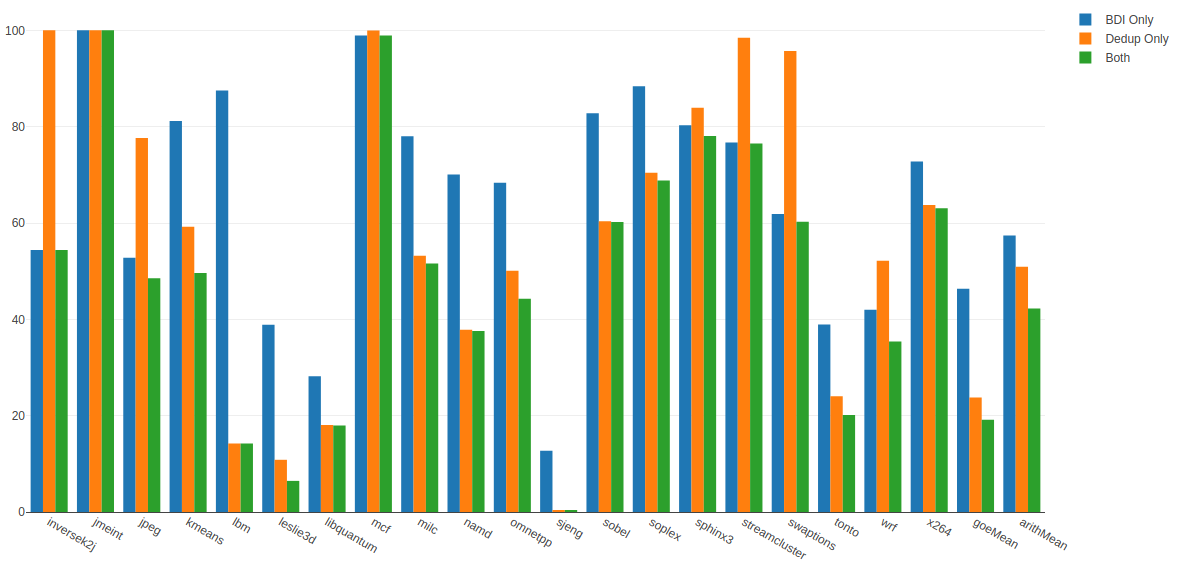
\includegraphics[width=\textwidth]{CompSize2.png}
    \end{subfigure}
    \caption[Size after compression]{The figure shows the size of data in a cache after using compression. BDI, Dedup, and a combination of both is shown.}
    \label{fig:CompSize}
\end{figure}
Nevertheless, combining BDI and Deduplication can still outperform each of them on its own. Figure \ref{fig:CompSize} shows the compressed data size when using BDI, Dedup, and Dedup+BDI. In its worst case Dedup+BDI performs the same as the best out of Dedup and BDI, in most cases it compresses even more on both. Note that the experiments used to create Figure \ref{fig:CompSize} are done statically on cache dumps and thus are completely missing the time dimension and its effect on compression. As time passes more requests to data lines can occur, with more requests the probability that compression can occur increases allowing for better compression.
